\section{Social Sustainability}
To define which are the relevant indicators for social sustainability, both in terms of quality of service for customers and as a workplace, it is possible to start from the SDGs listed in the introduction.

\begin{minipage}[c]{0.2\textwidth}
    
\includegraphics[width=\textwidth]{Images/Social_sustainability/1_no_poverty.png}
\end{minipage}
\begin{minipage}[c]{0.8\textwidth}
    According to the 1.3 SDG to be able to defeat poverty , the salaries must be adjusted to the job position according the national collective labour agreement. To monitor this aspect is useful to consider the following KPI: average salary level in proportion to the national collective labour agreement.
\end{minipage}
\hfill



\begin{minipage}[c]{0.2\textwidth}
    
\includegraphics[width=\textwidth]{Images/Social_sustainability/3_helth.png}
\end{minipage}
\begin{minipage}[c]{0.8\textwidth}
    The 3.6 SDG has the goal to halve the number of deaths and injuries from road traffic accidents worldwide by 2020. To monitor this aspect the following KPIs can be considered:
\begin{itemize}
    \item Number of injuries and deaths caused by road accidents
    \item Number of road accidents
\end{itemize}
\end{minipage}
\hfill

\begin{minipage}[c]{0.2\textwidth}
    
\includegraphics[width=\textwidth]{Images/Social_sustainability/4_education.png}
\end{minipage}
\begin{minipage}[c]{0.8\textwidth}
The 4.4 SDG emphasises the importance of training education in workplace in order to have always better quality of service and to increase safety of workers and clients.
\begin{itemize}
    \item Training hours per capita for traveling and non-traveling personnel
    \item \% Employees who received an evaluation during the year
\end{itemize}
\end{minipage}
\hfill

\begin{minipage}[c]{0.2\textwidth}
    
\includegraphics[width=\textwidth]{Images/Social_sustainability/5_gender.png}
\end{minipage}
\begin{minipage}[c]{0.8\textwidth}
Forms of discrimination and gender disparities are to be considered both transport service customers (5.1 SDG) and company employees (5.5 SDG). Some reference indicators to consider measuring the gender equity are the following:
\begin{itemize}
    \item \% female passengers: this information can be collected easily if the passenger register on the website or on the application of the company 
    \item Number of assaults and violence to women on buses
    \item \% women in management area: more importance on the women full and effective participation and equal leadership opportunities at all levels of decision-making in political, economic and public life
    \item \% women with a permanent contract 
    \item Ratio between training hour for woman and men
\end{itemize}
\end{minipage}
\hfill


\begin{minipage}[c]{0.2\textwidth}
    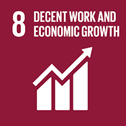
\includegraphics[width=\textwidth]{Images/Social_sustainability/8_work.png}
\end{minipage}
\begin{minipage}[c]{0.8\textwidth}
The 8.2 SDG  stresses the importance to achieve higher levels of economic productivity through diversification, technological updating and innovation, including through a focus on high value-added sectors and labour-intensive sectors. An element to obtain this result is to increase the quality of service.
\end{minipage}
\hfill

Quality of the service has become an element more and more important, for this reason is necessary to define the right KPI to measure the quality of the service and to know how to improve it. The analysis of service quality is of vital importance for both operators and public transport authorities because it plays a key role in attracting new passengers from private cars to the public transport system. The quality of the service depends on many factors; one important factor that become more significant in the last years with the Covid pandemic is the cleaning. The cleaning requirements by the PTA has changed and become stricter.

As reported in the document Carta della mobilità,  the quality of the service can be perceived through a series of fundamental factors that characterize the quality of each aspect of the trip (e.g. travel safety, regularity of the service, cleanliness and hygienic conditions of the vehicles, etc.) and, within each of these, by specific quality indicators (for example for travel safety: number of accidents, age of vehicles) which represent the performance levels of the service provided.

Each factor and quality indicator are associated with a value (which expresses the level of quality of the service actually provided) and a target set each year by the Company providing the service.

The data on customer satisfaction are collected, in accordance with the provisions of the service contracts, with surveys carried out every six months by an external market research company through response surveys. 

More in detail the surveys  analyse the following aspects with their respective KPIs:
\begin{itemize}
    \item Safety of the trip
\begin{itemize}
    \item	Accidents of the vehicles
    \item Passive accidents
    \item Age of vehicles
    \item Total perceived safety of the trip
\end{itemize}
    \item Personal and property safety
    \begin{itemize}
        \item	Complaints (theft and harassment)
        \item Total perceived personal safety
    \end{itemize}
    \item Regularity and punctuality of the service
    \begin{itemize}
        \item 	Regularity of the service
        \item Frequency of rides
        \item Commercial speed
        \item Punctuality in rush hours
        \item Punctuality in non-rush hours
        \item Total perceived regularity of the service
    \end{itemize}
    \item	Comfort and cleanliness of the buses
    \begin{itemize}
        \item Crowding in rush hours 
        \item Crowding in non-rush hours 
        \item Air conditioning
        \item Low-floor bus
        \item Additional services (mobile platform, wheelchair anchoring)
        \item Total perceived comfort
        \item Ordinary cleaning
        \item Extraordinary cleaning
        \item Cleaning of bus stations
        \item Total perceived cleanliness
    \end{itemize}
    \item Information and service to users
    \begin{itemize}
        \item Timeliness
        \item Internal visual devices
        \item Timetable at bus stops
        \item Point of sales of tickets
        \item Feedback to complaints
        \item Total perceived information and services
    \end{itemize}
    \item Relational aspects
        \begin{itemize}
            \item         Total perceived relational aspects
        \end{itemize}
    \item Attention to environment
        \begin{itemize}
            \item Electric or hybrid vehicles 
            \item Use of eco-fuels
            \item Vehicles Euro 3-4
            \item Vehicles Euro 4 and more
            \item Total perceived attention to environment
        \end{itemize}
\end{itemize}

The KPIs are reported in the following figure \ref{fig:kpis}, with a value form 0 (worst situation) to 4 (optimal situation). In 2019 there was an improvement in all indicators, except for the perceived security. For the 2020 the data are not available because the surveys were not carried out due to the Covid pandemic.


\begin{figure}[h]
    \centering
    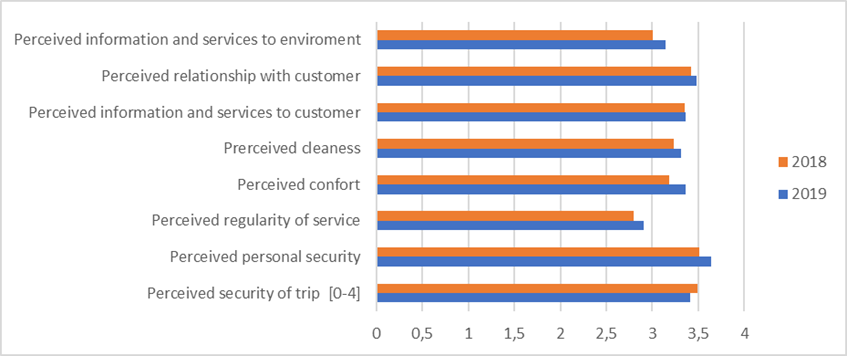
\includegraphics[width=0.9\textwidth]{Images/Social_sustainability/graph.png}
    \caption{KPIs}
    \label{fig:kpis}
\end{figure}
The importance of the cleaning is confirmed in the service contract which establishes penalties in case of:
\begin{itemize}
    \item failure to comply the frequency and/ or cycles in relation to the individual types of intervention (both for ordinary and extraordinary cleaning of the fleet and infrastructure and network systems open to the public).
    \item Insufficient cleaning of the bus (both for ordinary and extraordinary cleaning of the fleet and infrastructure and network systems open to the public).
\end{itemize}
·	


The main requirements for the cleaning are:
\begin{itemize}
    \item	daily cleaning (ordinary cleaning): it consists of removing the filth produced by the passengers, cleaning of cockpit, floor and handrails (about 10-15 min per bus);
    \item monthly cleaning (extraordinary cleaning): it is a deeper cleaning; special products must be used to remove dirt (generally it takes at least 30-40 min per bus)
    \item half yearly cleaning: vehicles are subjected to an antibacterial sanitization and disinfestation cycle 
    \item Nowadays, due to the pandemic situation, the consortium has introduced from March 2020 sanitation interventions with disinfection and sanitization in particular of the surfaces and passenger support points. Also, every fifteen days during the periodic cleaning interventions are performed cleaning by ionization
\end{itemize}


As shown in the results reported in Carta della mobilità, the customer satisfaction surveys (CSS) provide many information on the level of quality of a public transport service.
In addition with the new technologies it is possible to measure:
\begin{itemize}
    \item Regularity and punctuality with AVM
    \item Crowding indicator and possibility of sitting during the journey with passenger counters technology
\end{itemize}

\begin{minipage}[c]{0.2\textwidth}
    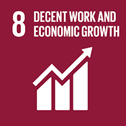
\includegraphics[width=\textwidth]{Images/Social_sustainability/8_work.png}
\end{minipage}
\begin{minipage}[c]{0.8\textwidth}
The 8 SDG remark the importance of an equal and fair salary for all workers, including young people and people with disabilities and the importance to reduce the percentage of unemployed young people who do not follow a course of study or who do not follow training courses. Another aspects is the protection of labour rights and promotion a safe and secure working environment for all workers, including migrant workers, especially migrant women, and those in precarious work. The KPIs useful for this aspect are:
\begin{itemize}
    \item \% employees with permanent contract
    \item \% employees under 35 
    \item \% turnover rate
    \item Frequency of injuries of workers
    \item Index of severity of injuries
    \item Number of hours of training on safety and health
    \item \% employees registered with trade unions
    \item Number of hours of trade union assemblies
    \item Complaints related to work practices
\end{itemize}
\end{minipage}

\begin{minipage}[c]{0.2\textwidth}
    
\includegraphics[width=\textwidth]{Images/Social_sustainability/9_industry.png}
\end{minipage}
\begin{minipage}[c]{0.8\textwidth}
The importance of access to information and communication technologies is remarked by the 9.6 SDG. A transport company to achieve that goal could provide a company phone to employees

\begin{itemize}
    \item \% Employees with company phone with application used by the company
\end{itemize}
\end{minipage}

\begin{minipage}[c]{0.2\textwidth}
    
\includegraphics[width=\textwidth]{Images/Social_sustainability/16_peace.png}
\end{minipage}
\begin{minipage}[c]{0.8\textwidth}
The has the goal by 2030, to reduce illicit financing and arms trafficking, enhance the recovery and return of stolen assets and fight all forms of organized crime, reduce corruption and all its forms (16.4), Develop effective, accountable and transparent institutions at all levels (16.6).
To monitor fare evasion, corruption and arms trafficking:
\begin{itemize}
    \item	Number of passengers checked
    \item Number of clients connected on social network
    \item Number of accesses to the site
    \item Courtesy of drivers$\rightarrow$ this information is already collected with the customer satisfaction survey
    \item Number of info point in the area 
    \item Number of point of sales of tickets in the area
\end{itemize}
\end{minipage}
\\
\begin{minipage}[c]{0.2\textwidth}
    
\includegraphics[width=\textwidth]{Images/Social_sustainability/17_partnerships.png}
\end{minipage}
\begin{minipage}[c]{0.8\textwidth}
The 17.13 and 17.17 remind the importance of coordination, coherence to achieve goals global macro-economic stability. 
\begin{itemize}
    \item Number of trade union agreements signed in recent years
    \item Number of partnerships with university
\end{itemize}
\end{minipage}